\documentclass[12pt,twoside]{article}
\usepackage[dvipsnames]{xcolor}
\usepackage{tikz,graphicx,amsmath,amsfonts,amscd,amssymb,bm,cite,epsfig,epsf,url}
\usepackage[hang,flushmargin]{footmisc}
\usepackage[colorlinks=true,urlcolor=blue,citecolor=blue]{hyperref}
\usepackage{amsthm,multirow,wasysym,appendix}
\usepackage{array,subcaption} 
% \usepackage[small,bf]{caption}
\usepackage{bbm}
\usepackage{pgfplots}
\usetikzlibrary{spy}
\usepgfplotslibrary{external}
\usepgfplotslibrary{fillbetween}
\usetikzlibrary{arrows,automata}
\usepackage{thmtools}
\usepackage{blkarray} 
\usepackage{textcomp}
\usepackage[left=0.8in,right=1.0in,top=1.0in,bottom=1.0in]{geometry}

\input{macros}

\begin{document}

\begin{center}
{\large{\textbf{Homework 3}} } \vspace{0.2cm}\\
Due October 8 at 11 pm
\\
\end{center}
\input{hwstatement.tex}\\

\begin{enumerate}

\item (Fish)
A biologist is studying a rare species of fish. She captures four individuals and measures their weights, which are 5, 8, 5 and 6 kg.
\begin{enumerate}
\item
What is the empirical conditional probability that a fish weighs more than 7 kg given that they weigh more than 6 kg? 
\item Plot an estimate of the pdf of the fish weight using kernel density estimation with a rectangular kernel of width 2.
\item What is the conditional probability that a fish weighs more than 7 kg given that they weigh more than 6 kg according to your estimated pdf?
\end{enumerate}

\item (Nuclear power plant)
The random variable $\rt$ with the following pdf
\begin{figure}[h]
\begin{center}
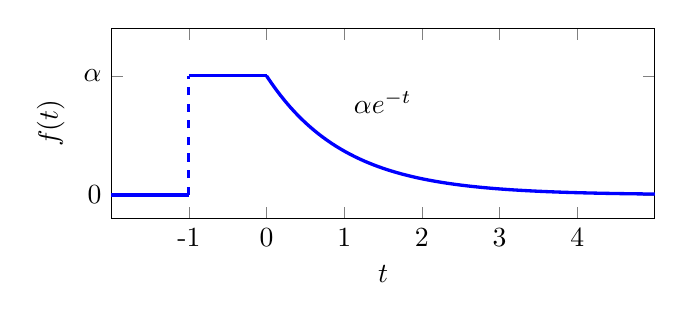
\begin{tikzpicture}
\begin{axis}[xmin= -2, xmax=5, ymin=-0.1, ymax=0.7, xlabel=$t$,
ylabel=$f_{\rt}(t)$,height=4cm,
width=0.7\textwidth,
xticklabels={-1,0,...,4}, xtick={-1,0,1,...,4},
yticklabels={0,$\alpha$}, ytick={0,0.5}]
%\addplot+[ycomb, blue, very thick, samples=2] coordinates {(0,1)(1,1)};
\addplot[blue, very thick, samples=2] coordinates {(-2,0)(-1,0)};
\addplot[blue, very thick, samples=2] coordinates {(-1,0.5)(0,0.5)};
%\addplot[dashed,blue, very thick, samples=2] coordinates {(0,0)(0,0.5)};
\addplot[dashed, blue, very thick, samples=2] coordinates {(-1,0)(-1,0.5)};
\addplot[blue, very thick, domain=0:6, samples=101] {0.5*exp(-x)};
\node at (axis cs:1,0.3) [anchor=south west] {$\alpha e^{-t}$};
%\addplot[dashed,blue, very thick, samples=2] coordinates {(0,0)(0,0.5)};
\end{axis}
\end{tikzpicture} 
\end{center}
\end{figure}\\
models the time at which there is a leak in a nuclear power plant. The pdf is constant during the time the station is built (between -1 and 0) and exponential with parameter 1 afterwards (from 0 to $+\infty$). 
\begin{enumerate}
\item Compute the value of the constant $\alpha$. 
\item Compute the cdf of $\rt$ and plot it.
\item Compute the pdf of $\rt$ conditioned on $\rt <0$.
\end{enumerate}

\item (Measurements)  
You have access to the readings of a device that indicates whether a radioactive particle has decayed. However you do not get a continuous reading, you get a reading every second. 
\begin{enumerate}
\item A reasonable model for the time the particle takes to decay is that it is a random variable with pdf
\begin{align}
f_{\rnd{t}}(t) := \begin{cases}
\lambda \exp(- \lambda t), \qquad \text{if $t\geq 0$},\\
0 \qquad \text{otherwise},
\end{cases}
\end{align}
where $\lambda$ is a fixed constant. Taking into account that the measurement device rounds up the time and outputs an integer number of seconds (if the time is $0.1$ it outputs 1, if it is 13.4 it outputs 14), compute the pmf of the reading from the device. What kind of random variable is this? 
\item What is the pdf of the error between your reading and the true time of decay?
\end{enumerate}

\item (Applying the cdf) The array in \texttt{samples.npy} contains $n := 1,000$ i.i.d. samples from a certain distribution. 
\begin{enumerate}
\item Compute the empirical cdf of the data $F_X$ and plot it. 
\item If you apply the empirical cdf to each data point $x_i$ , $1\leq i \leq n$, to obtain a new data point $y_i := F_X(x_i)$, what are the new data equal to? Does your answer depend on the distribution of the data?
\end{enumerate}
\end{enumerate}
\end{document}
